%%%\scalebox{1.2}{ 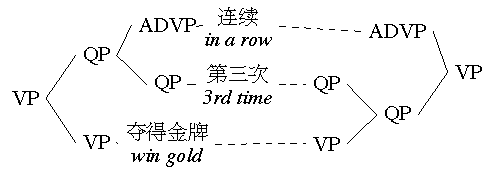
\includegraphics{figures/chinese-treemodatt} }

\begin{tikzpicture}
\tikzset{every tree node/.style={align=center}}
\Tree
[.VP
  [.ADVP 连续\\{in a row} ]
  [.\extranode{QP}
    [.QP 第三次\\{third time} ]
    [.VP 夺得金牌\\{win gold} ] ] ]
\end{tikzpicture}

\vspace{3mm}
(a) Parser output

\vspace{6mm}

\begin{tikzpicture}
\tikzset{every tree node/.style={align=center}}
\Tree
[.VP
  [.\missingnode{QP}
    [.ADVP 连续\\{in a row} ]
    [.QP 第三次\\{third time} ] ]
  [.VP 夺得金牌\\{win gold} ] ]
\end{tikzpicture}

\vspace{3mm}
(b) Gold parse
\derivspace
\caption[Error analysis example: Adverb and adjective modifier attachment (Chinese).]{ \label{fig:mod_att}
  \textbf{Modifier Attachment}: \glos{连续}{in a row} should modify only \glos{第三次}{third time}.
}
